% \pagebreak[4]
% \hspace*{1cm}
% \pagebreak[4]
% \hspace*{1cm}
% \pagebreak[4]

\chapter{Tổng quan}
\ifpdf
    \graphicspath{{Chapter1/Chapter1Figs/PNG/}{Chapter1/Chapter1Figs/PDF/}{Chapter1/Chapter1Figs/}}
\else
    \graphicspath{{Chapter1/Chapter1Figs/EPS/}{Chapter1/Chapter1Figs/}}
\fi
\markboth{\MakeUppercase{Chương \thechapter. Tổng quan}}{Chương \thechapter. Tổng quan}
\section{Đặt vấn đề}
Trong những năm gần đây, cùng với sự phát triển của công nghệ thông tin, các lĩnh vực liên quan đến kỹ thuật số cũng đang có tốc độ phát triển chóng mặt. Các thiết bị kỹ thuật số như máy ảnh, máy quay phim kỹ thuật số, camera số, điện thoại di động có chức năng chụp hình,... đang ngày càng phổ biến và không ngừng gia tăng về số lượng. Chính điều này đã làm sản sinh ra một lượng ảnh số khổng lồ. Do đó, nhu cầu truy vấn thông tin từ kho dữ liệu hình ảnh ngày càng bức thiết hơn bao giờ hết.

Để đáp ứng yêu cầu đó, rất nhiều hệ thống truy vấn ảnh đã ra đời. Với đầu vào là một hình ảnh có chứa đối tượng quan tâm, hệ thống sẽ trả về những hình ảnh có chứa đối tượng quan tâm trong kho dữ liệu ảnh có sẵn. Hình ảnh \ref{FigSystem} minh họa tổng quát cho một hệ thống truy vấn đối tượng trên ảnh.

\begin{figure}[!htbp]
  \begin{center}
    \leavevmode
    \ifpdf
      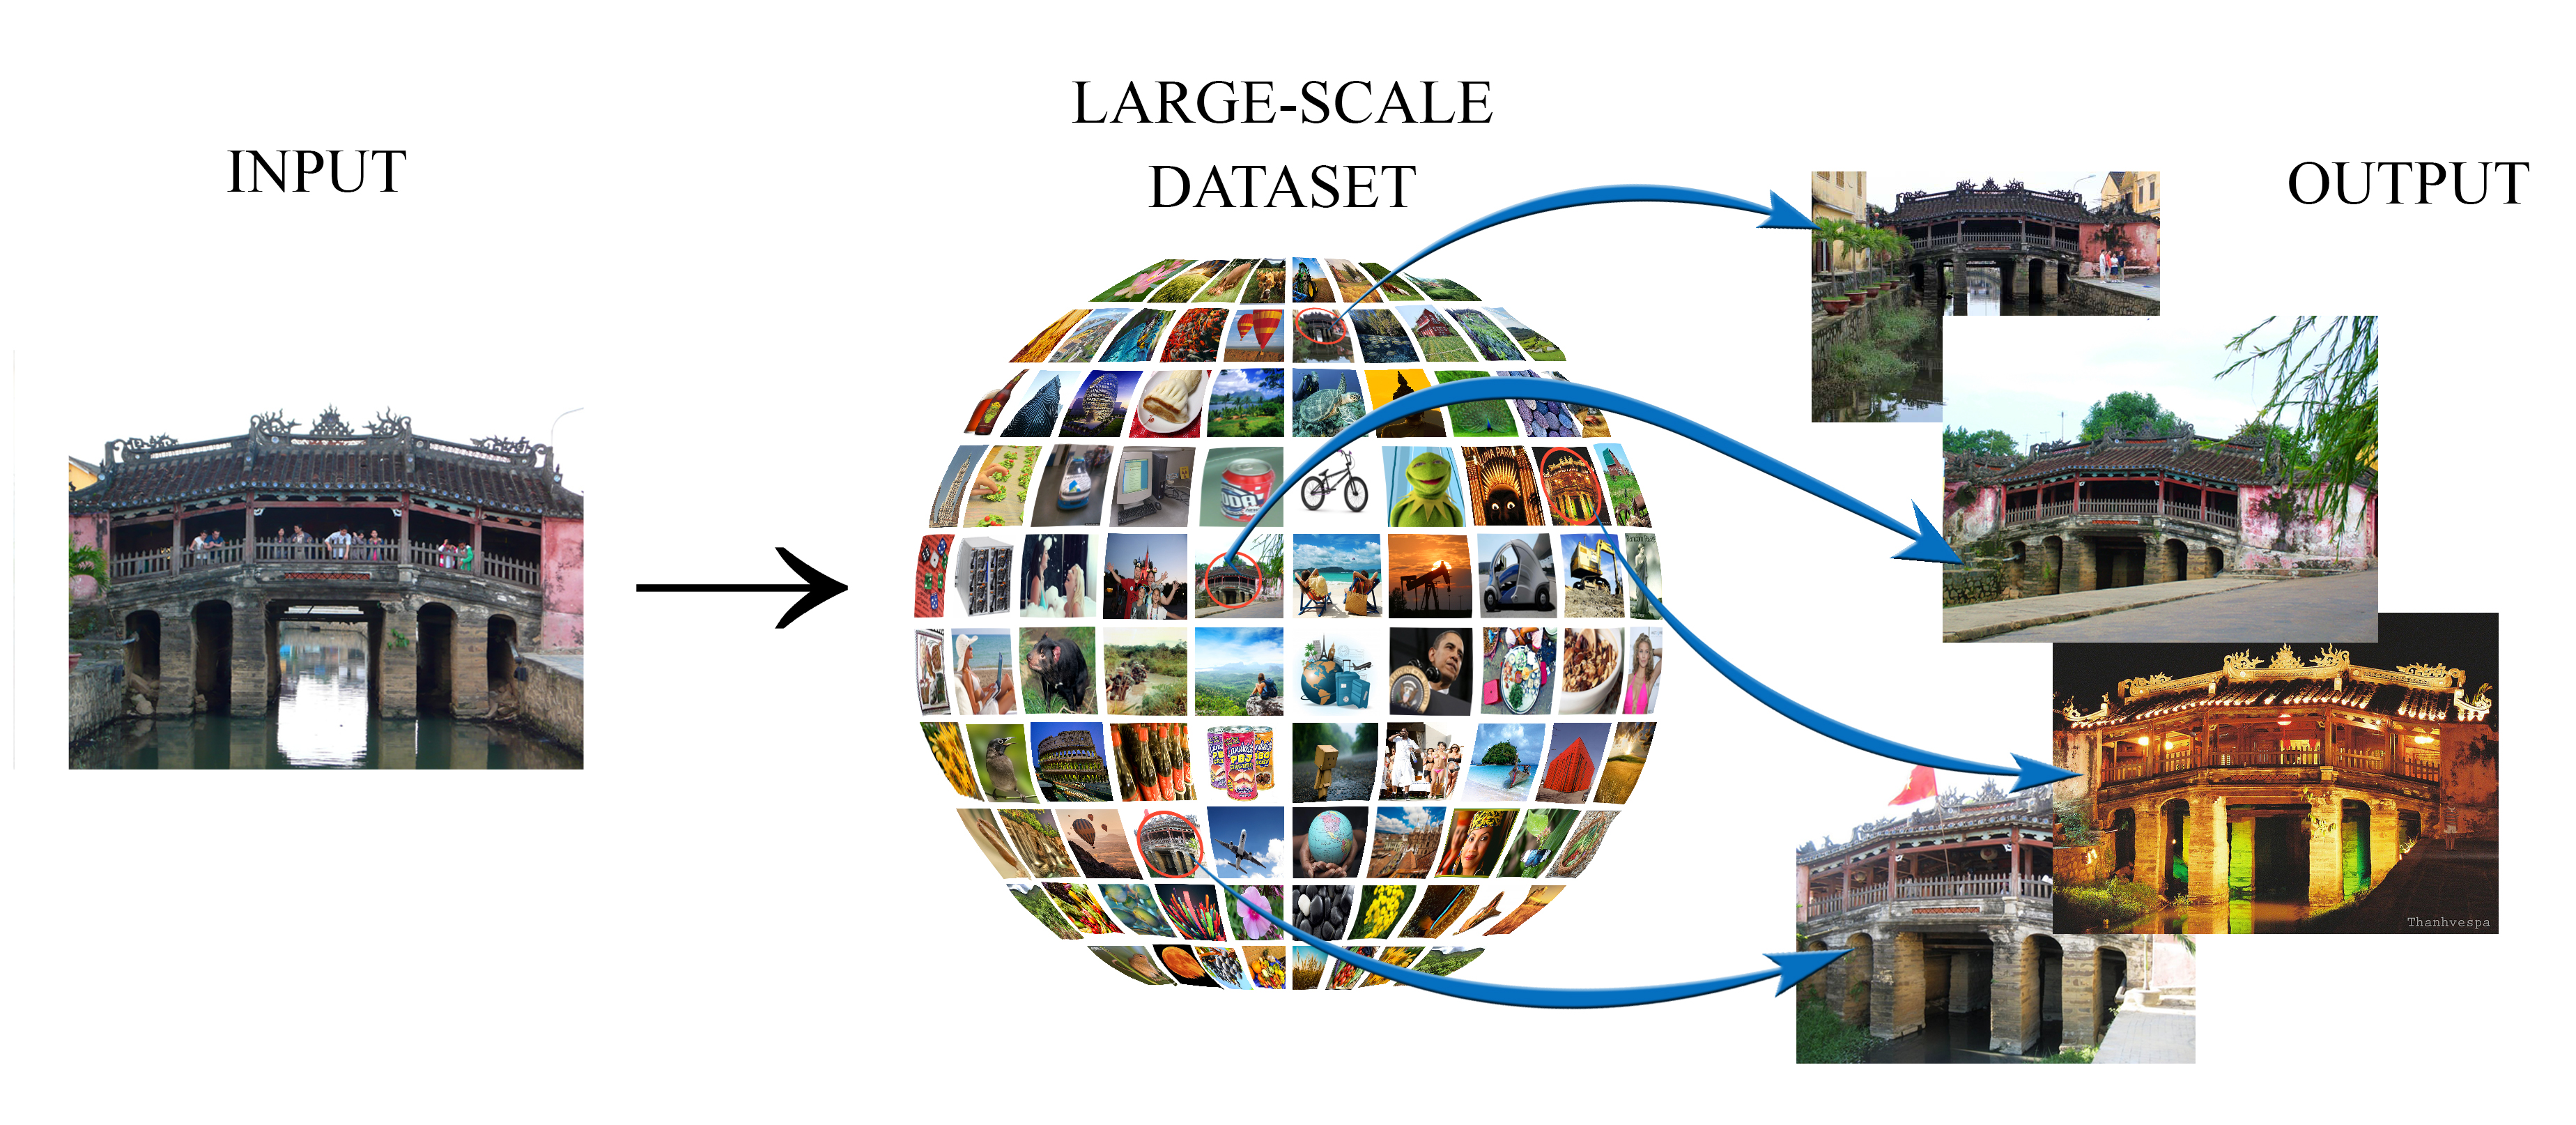
\includegraphics[scale=0.113]{retrievalSystem}
    \else
      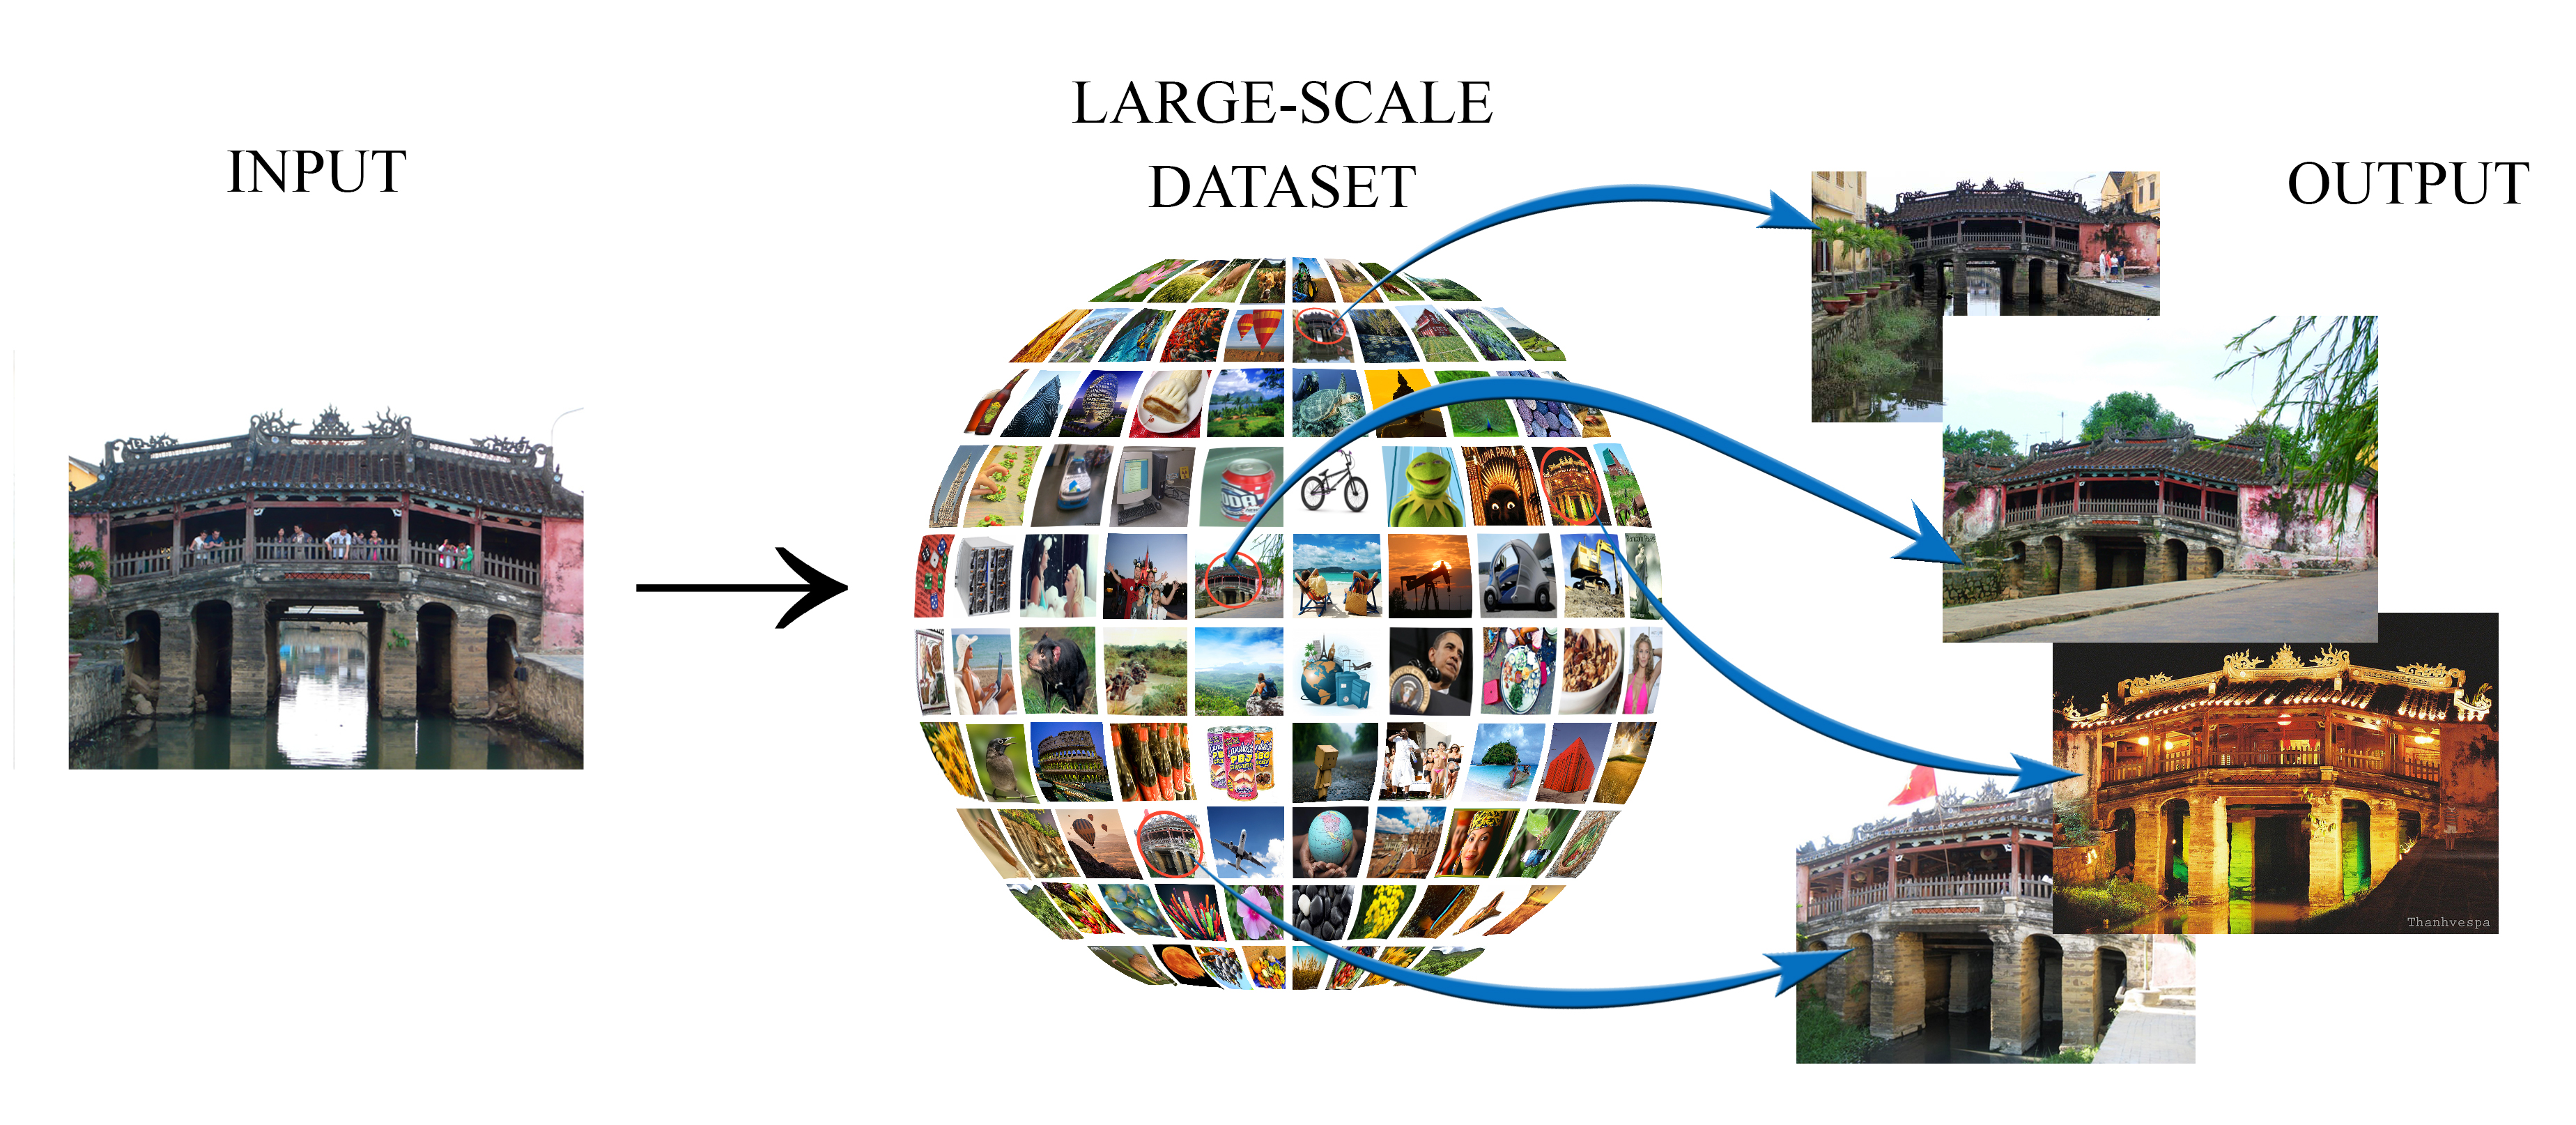
\includegraphics[scale=0.113]{retrievalSystem}
    \fi
    \caption[Ví dụ minh họa về bài toán tìm kiếm ảnh]{Ví dụ minh họa về bài toán tìm kiếm ảnh}
    \label{FigSystem}
  \end{center}
\end{figure} 

Những hệ thống truy vấn ảnh trên tập dữ liệu lớn có rất nhiều ứng dụng trong thực tế. Từ những ứng dụng phục vụ nhu cầu truy vấn thông tin hàng ngày cho tới những ứng dụng giúp quản lý kho dữ liệu lớn trong doanh nghiệp. Chúng tôi sẽ liệt kê sơ lược một vài ứng dụng của hệ thống này dưới đây.

\begin{itemize}
\renewcommand{\labelitemi}{$\ast$}
\item \textbf{Một vài hướng ứng dụng của hệ thống truy vấn ảnh}
\end{itemize}

Trong cuộc sống, ta có thể dễ dàng bắt gặp những ứng dụng vô cùng hữu ích của các hệ thống truy vấn đối tượng trên ảnh. Dưới đây là một vài hướng ứng dụng cụ thể:\\
\textbf{Tìm kiếm đối tượng, sản phẩm.} Với sự phổ biến của điện thoại thông minh và internet, một người có thể dễ dàng dùng điện thoại chụp một tấm hình và hỏi hệ thống về thông tin của đối tượng trong tấm hình đó. Ví dụ, tại một cửa hàng, một người mua hàng có thể tham khảo giá của một sản phẩm tại các cửa hàng khác; trong thư viện, một độc giả có thể tìm được những cuốn sách nào chứa hình ảnh mình quan tâm; khi đi thăm bảo tàng, du khách có thể tìm kiếm thêm thông tin về một hiện vật trong đó, v.v...\\
\textbf{Xác định địa điểm.} Vị trí địa lý của nơi chụp tấm hình cũng có thể được xác định bằng việc truy vấn thông tin của đối tượng trong hình từ những cơ sở dữ liệu lớn chứa hình ảnh và thông tin vị trí như Google Street View hay kho hình ảnh có lưu kèm thông tin GPS. Hệ thống này có thể là một giải pháp thay thế rẻ tiền cho các thiết bị có GPS. Chẳng hạn, khi một du khách đến một nơi mà anh ta chưa bao giờ đặt chân tới nhưng lại không GPS hay bản đồ, anh ta có thể chụp một tấm hình của một tòa nhà hay những cảnh tại nơi đó để xác định được vị trí chính xác của mình.\\
\textbf{Tìm kiếm và quản lý kho dữ liệu video.} Hàng ngày, một lượng lớn dữ liệu video được sinh ra và ta không thể nào quản lý hết được nội dung của chúng. Ví dụ, một đài truyền hình muốn tìm kiếm tất cả các đoạn quảng cáo có liên quan đến một nhãn hiệu sản phẩm mà họ đã từng phát trong vài năm gần đây hay ta muốn biết một đối tượng xuất hiện trong cảnh nào của một bộ phim, v.v... Bởi vì video được tạo nên từ các khung hình khác nhau nên một hệ thống truy vấn ảnh sẽ dễ dàng thực hiện điều này chỉ với một hình ảnh của đối tượng quan tâm.\\
\textbf{Sử dụng trong quảng cáo theo ngữ cảnh.} Rất nhiều công ty quảng cáo đặt màn hình tại nơi công cộng để quảng cáo cho các sản phẩm của mình nhưng các quảng cáo này chưa thực sự hướng người dùng và kém hiệu quả. Việc sử dụng một hệ thống có thể quảng cáo theo ngữ cảnh và hướng đúng đối tượng người dùng sẽ giúp việc quảng cáo hiệu quả hơn. Ví dụ, một camera trong thang máy có thể tự động tìm kiếm thông tin về những sản phẩm người đi thang máy đang dùng như nhãn hiệu chai nước họ đang uống, nhãn hiệu quần áo họ đang mặc,... để lựa chọn được những quảng cáo phù hợp với đối tượng người dùng và phát trên màn hình.\\
\textbf{Hỗ trợ cho các hệ thống thị giác máy tính khác.} Hệ thống truy vấn đối tượng có thể được dùng để hỗ trợ cho các hệ thống thị giác máy tính khác. Một ví dụ điển hình là hệ thống tự động tái tạo hình ảnh ba chiều sẽ cần gom cụm các hình ảnh của cùng một đối tượng từ một tập dữ liệu lớn.\\
\section{Thách thức}
 Để giải quyết bài toán truy vấn đối tượng trên tập dữ liệu ảnh lớn, có rất nhiều vấn đề thách thức phải giải quyết. Dưới đây chúng tôi sẽ trình bày những thách thức chính trong bài toán này:\\
 \begin{figure}[!htbp]
  \begin{center}
    \leavevmode
    \ifpdf
      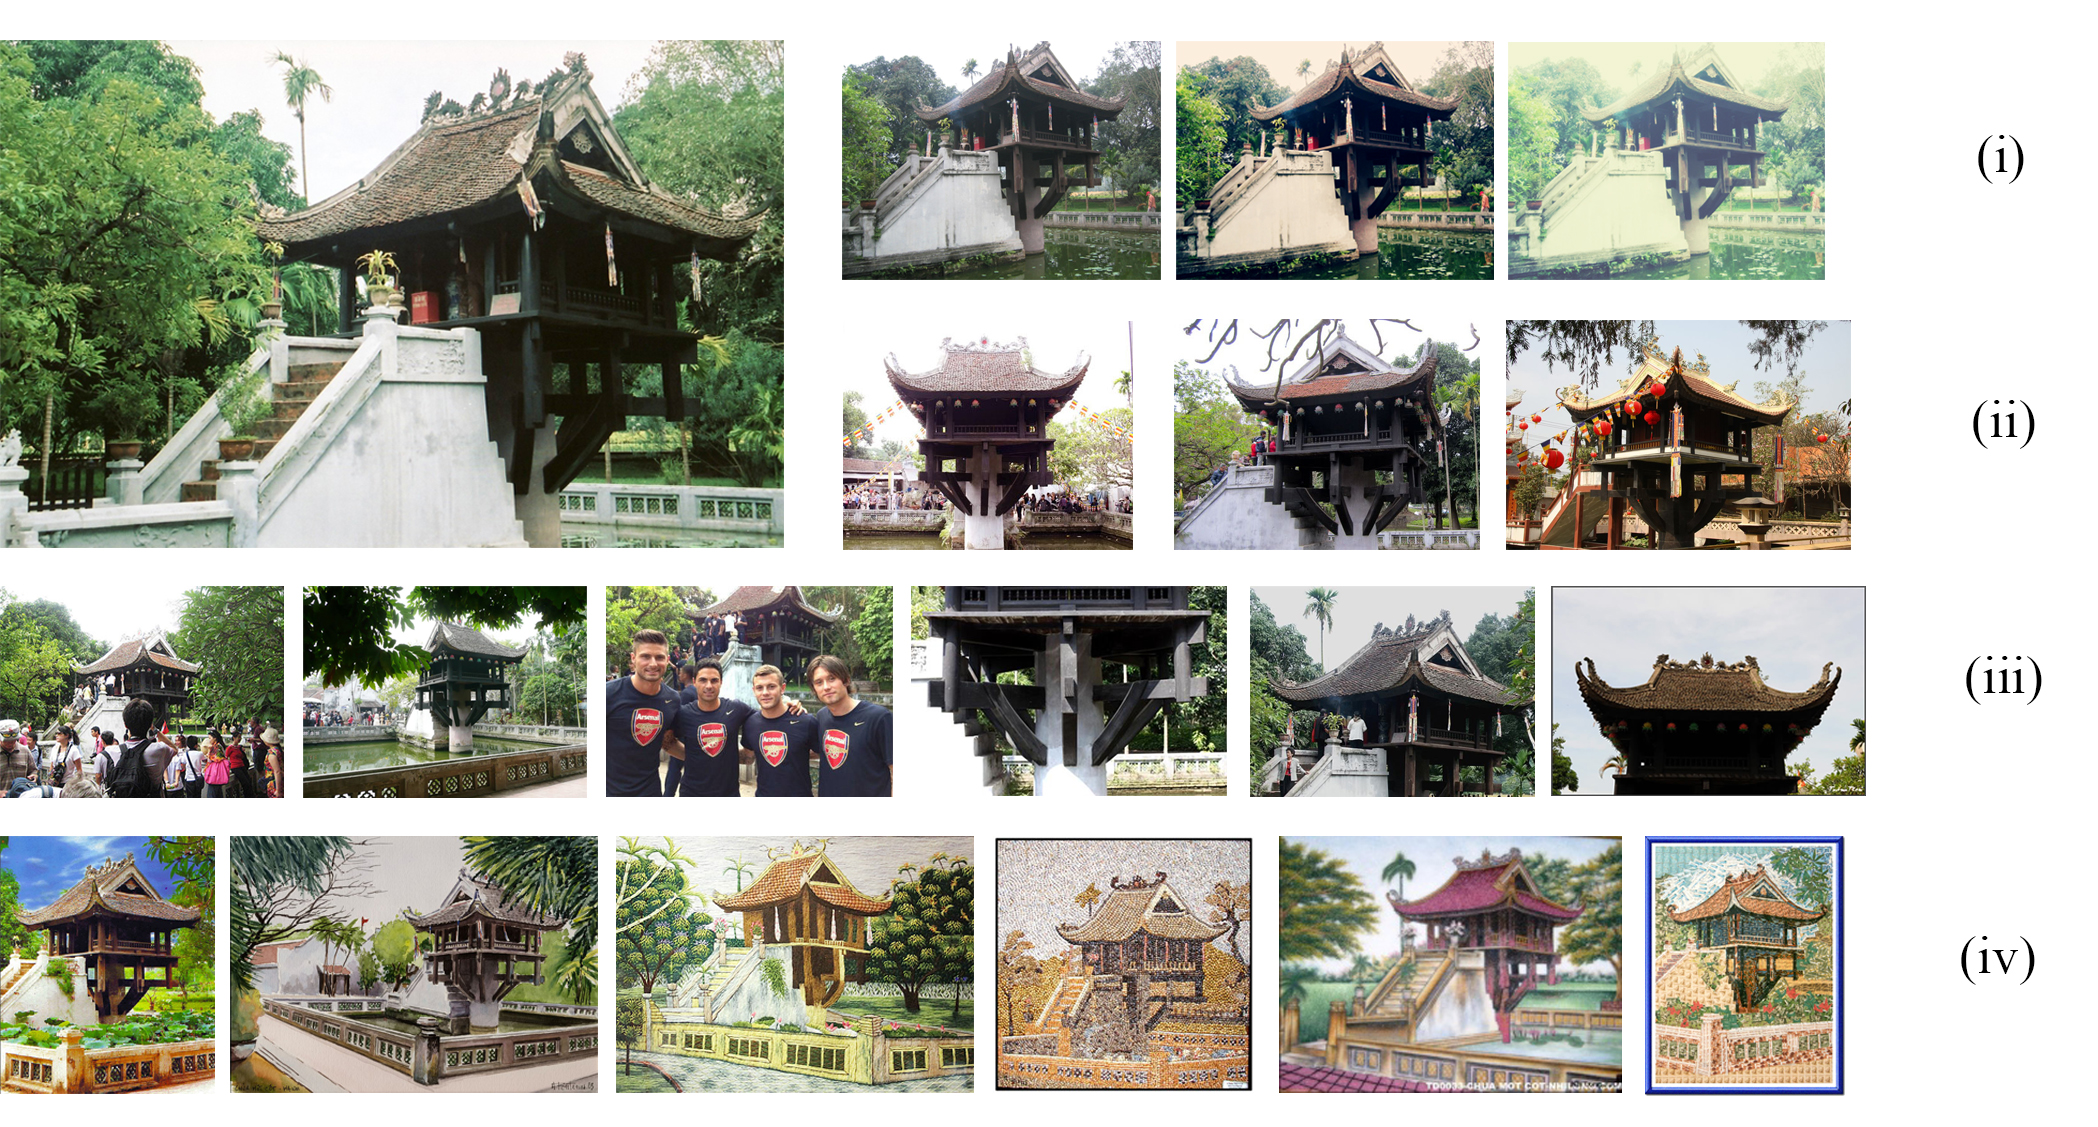
\includegraphics[scale=0.20]{chuaMotCot}
    \else
      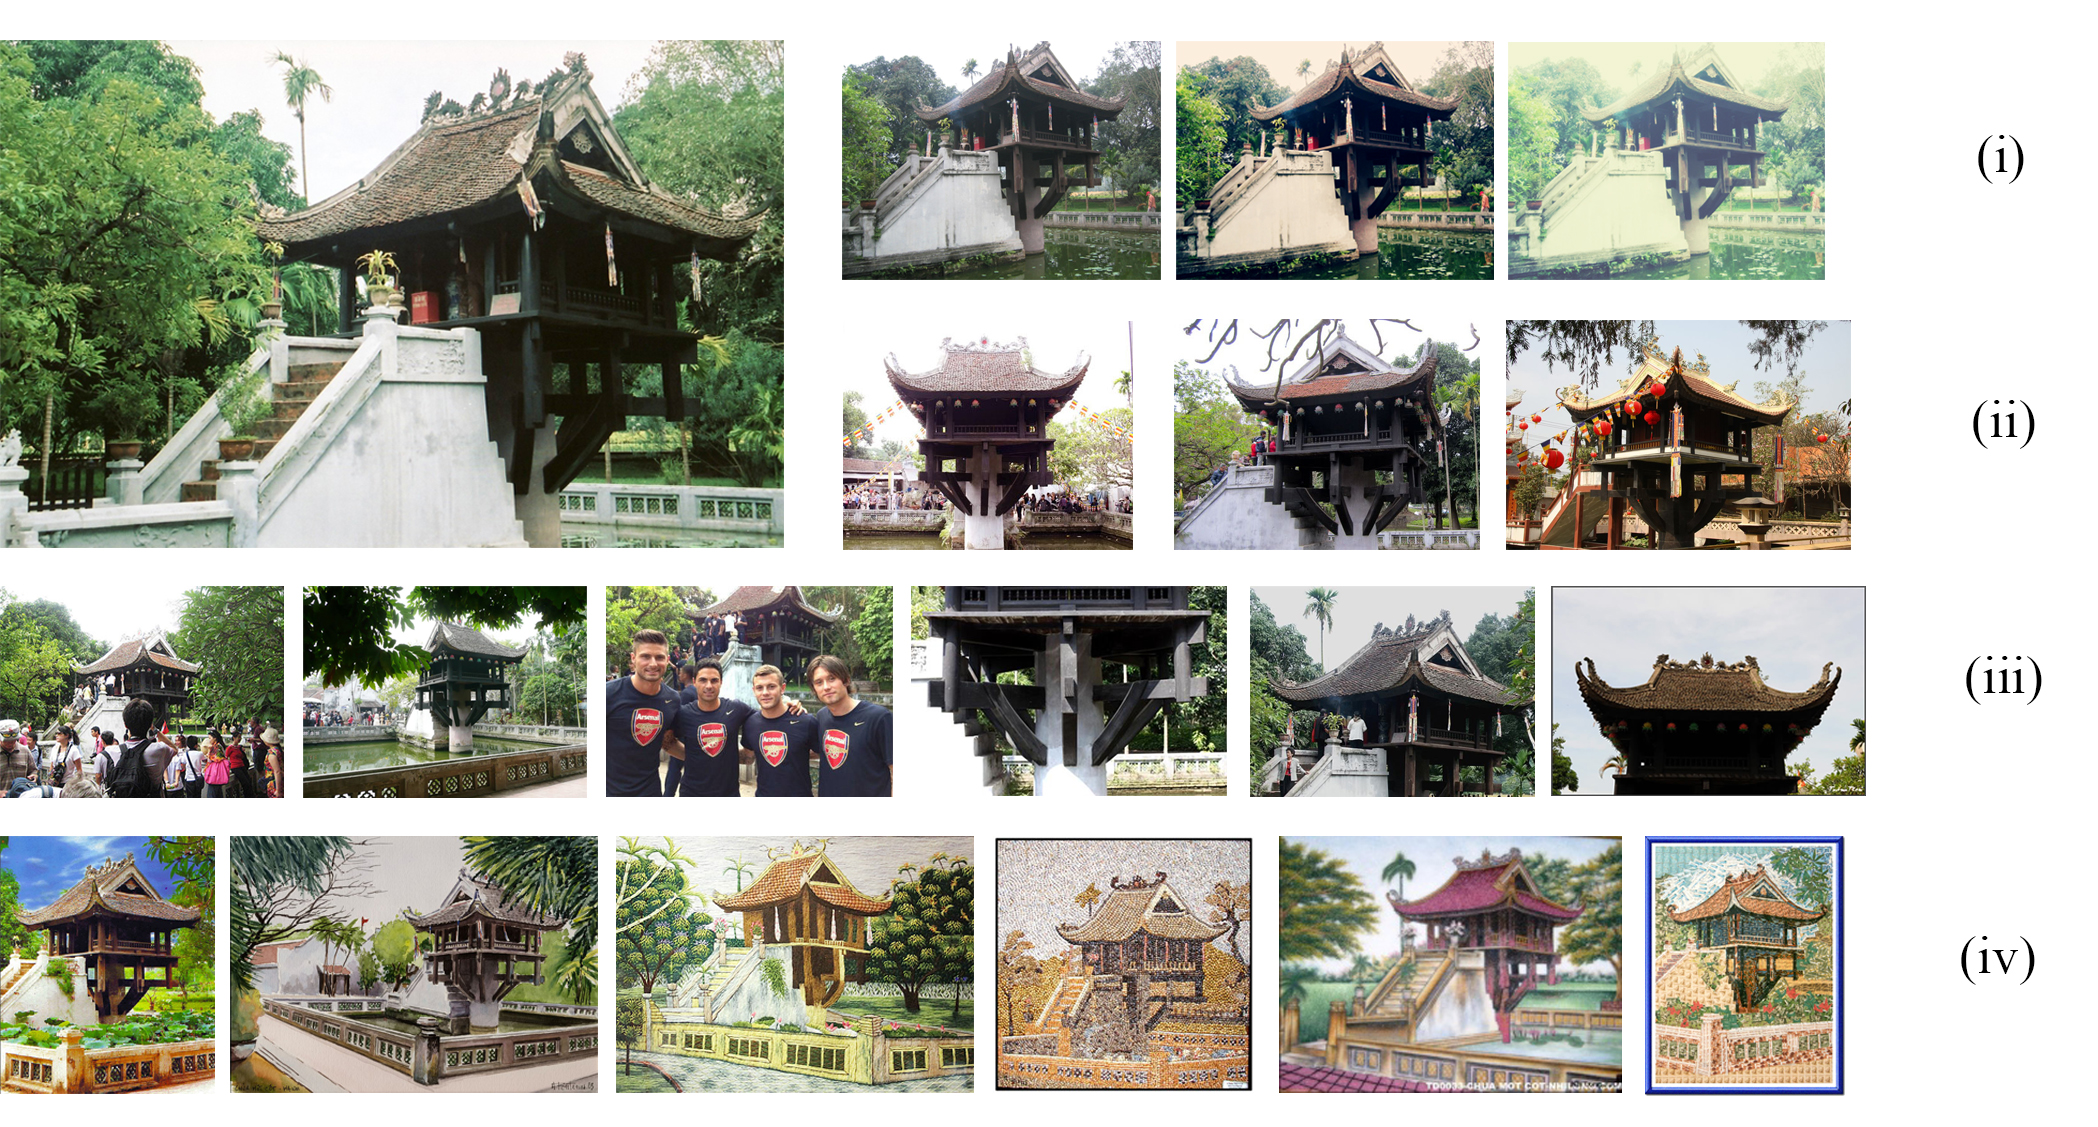
\includegraphics[scale=0.20]{chuaMotCot}
    \fi
    \caption[Những thay đổi bề ngoài của đối tượng trên ảnh]{\textbf{Những thay đổi bề ngoài của đối tượng trên ảnh.} (i) Hình ảnh đối tượng trong các điều kiện chiếu sáng khác nhau. (ii) Hình ảnh đối tượng dưới các góc chụp khác nhau. (iii) Đối tượng bị che khuất hay hình ảnh đối tượng bị cắt ghép. (iv) Hình ảnh đối tượng trong các ấn phẩm, bản in, bản vẽ. (Những hình ảnh này được lấy từ Google Image Search với query là "chùa Một Cột").}
    \label{FigTemple}
  \end{center}
\end{figure} 
\textbf{Sự biến đổi bề ngoài của đối tượng trong hình ảnh.} Một hệ thống truy vấn đối tượng trên hình ảnh cần phải trả về được các hình ảnh có chứa đối tượng quan tâm bất chấp mọi thay đổi trên bên ngoài của đối tượng. Những thay đổi đó có thể đến từ rất nhiều nguyên nhân khác nhau. Đó có thể do tác động từ các yếu tố bên ngoài khi chụp hình như điều kiện chiếu sáng, góc chụp của camera hay những tùy chỉnh khác nhau của các camera về độ tương phản, độ phân giải, màu sắc,... Cùng với đó là những hình ảnh của đối tượng được chụp với góc xoay, kích thước hình hay tỉ lệ khác nhau. Hoặc có những trường hợp đối tượng bị che khuất, cắt ghép, v.v... hoặc đối tượng được thể hiện trên các ấn phẩm, bản in, bản vẽ nên bị thay đổi về màu sắc và chi tiết. Một vài dạng thay đổi kể trên được thể hiện qua Hình \ref{FigTemple}. Còn một trường hợp nữa là do những thay đổi từ chính bản thân đối tượng do các điều kiện bên ngoài ví dụ như đối tượng bị cũ đi hay bị xuống cấp theo thời gian.\\
 \textbf{Kích cỡ của tập dữ liệu lớn.} Tập dữ liệu hình ảnh lớn thường bao gồm hàng triệu bức ảnh, vậy nên để người dùng có thể tương tác trực tiếp với hệ thống thông qua một thiết bị phía client như điện thoại di động thì đòi hỏi truy vấn phải được trả về trong thời gian ngắn chấp nhận được. Do đó cần phải có một giải pháp tìm kiếm hiệu quả, chi phí thấp. Đồng thời những hình ảnh cũng phải được xử lý để lưu trữ sao cho tiết kiệm nhất cho phù hợp với nhiều thiết bị với tài nguyên tính toán khác nhau.\\
 
\section{Mục tiêu, đối tượng và phạm vi nghiên cứu}
\subsection{Mục tiêu}
Mục tiêu của khóa luận này nhằm xây dựng một hệ thống truy vấn đối tượng trên ảnh từ tập dữ liệu lớn, trong đó quá trình truy vấn hoàn toàn dựa trên nội dung của ảnh. Hệ thống cần có độ chính xác tương đương hoặc tốt hơn so với các giải pháp phổ biến nhất hiện nay trong khi vẫn có thể duy trì tốc độ phản hồi cao. Hệ thống này tập trung vào giải quyết vấn đề về tìm kiếm một đối tượng cụ thể. Mục đích của hệ thống không phải là trả về những hình ảnh chụp gần giống nhau như chụp trong cùng một khung cảnh hay cùng thuộc một loại đối tượng mà là trả về những hình ảnh có chứa chính xác đối tượng cần tìm. Ví dụ như khi đưa vào một bức hình có chứa Nhà thờ Đức Bà, kết quả trả về sẽ những bức hình có chứa nhà thờ Đức Bà chứ không phải trả về những nhà thờ có kiến trúc hay có không gian bao quanh giống với Nhà thờ Đức Bà.

\subsection{Đối tượng nghiên cứu}
Đối tượng nghiên cứu trong khóa luận này là các hệ thống truy vấn ảnh, trong đó tập trung vào các giải pháp cho rút trích các đặc trưng hình ảnh, các phương pháp biểu diễn hình ảnh trên máy tính để phục vụ cho mục đích truy vấn, các kỹ thuật giúp tăng tốc quá trình truy vấn, các phương pháp sử dụng thông tin không gian ảnh trong bài toán truy vấn để nâng cao độ chính xác của truy vấn. Cùng với đó là các phương pháp và các bộ dữ liệu chuẩn được sử dụng rộng rãi trên thế giới để đánh giá kết quả của phương pháp đề xuất cho bài toán truy vấn.

\subsection{Phạm vi nghiên cứu}
Đề tài tập trung nghiên cứu những vấn đề chính sau:

-- Các kiến thức nền tảng trong lĩnh vực xử lý ảnh về phát hiện và rút trích các đặc trưng trên ảnh.

-- Các kỹ thuật biểu diễn hình ảnh.

-- Các kỹ thuật, phương pháp nâng cao trong bài toán truy vấn ảnh: kỹ thuật đánh chỉ mục, kỹ thuật so khớp hình ảnh, phương pháp xếp hạng hình ảnh.

-- Các bộ dữ liệu chuẩn để đánh giá hiệu suất của các phương pháp cho bài toán tìm kiếm đối tượng trên ảnh. 


\section{Cấu trúc luận văn}
Trong phần này, chúng tôi sẽ trình bày cấu trúc phần còn lại của luận văn và những vấn đề được thảo luận ở phần kế tiếp. Các nội dung sẽ được trình bày ở phần kế tiếp bao gồm:\\
 \textbf{Các công trình liên quan.} Chúng tôi sẽ giới thiệu tổng quan về các công trình nghiên cứu có liên quan tới bài toán truy vấn ảnh, các hướng tiếp cận và bàn luận chi tiết về từng công trình trong Chương \ref{chapter:related}.\\
 \textbf{Phương pháp đề xuất.} Chúng tôi đề xuất một phương pháp nhằm nâng cao hiệu suất của các hệ thống truy vấn đối tượng bằng cách tích hợp thông tin về phân bố trong không gian của các điểm đặc trưng vào phương pháp đánh chỉ mục ngược (inverted index). Chi tiết về phương pháp đề xuất được trình bày trong Chương \ref{chapter:proposed}.\\
 \textbf{Thí nghiệm.} Để đánh giá hiệu quả của phương pháp đề xuất và so sánh với các phương pháp khác, chúng tôi tiến hành thí nghiệm trên ba bộ dữ liệu chuẩn là Oxford 5K, Paris 6K và Oxford 100K. Kết quả được tính bằng phương pháp mean Average Precision (mAP). Chương \ref{chapter:experiment} sẽ trình bày chi tiết về các bộ dữ liệu, việc cài đặt thí nghiệm và kết quả thí nghiệm.\\
 \textbf{Xây dựng ứng dụng.} Chương \ref{chapter:application} tập trung vào việc thiết kế và cài đặt ứng dụng truy vấn đối tượng trên ảnh. Ứng dụng được xây dựng trên nền tảng mobile và tương tác với server thông qua webservice. Việc xây dựng ứng dụng nhằm chứng minh tính thực tế của đề tài.\\
 \textbf{Tổng kết.} Trong Chương \ref{chapter:summarize}, chúng tôi sẽ tổng kết, bàn luận thêm về phương pháp đề xuất và những đề xuất cải tiến, mở rộng để nâng cao hiệu suất của hệ thống trong thời gian tới.
 
